\documentclass[upright, contnum]{umemoria}
\depto{DEPARTAMENTO DE CIENCIAS DE LA COMPUTACI�N}
\author{WILLY ADOLFO MAIKOWSKI CORREA}
\title{REDISE�O E IMPLEMENTACI�N DE UN SISTEMA DE RECUENTO DE UNIDADES DOCENTES PARA LA FACULTAD DE CIENCIAS F�SICAS Y MATEM�TICAS}
\auspicio{}
\date{DICIEMBRE 2015}
\guia{PATRICIO POBLETE OLIVARES}
\carrera{INGENIERO CIVIL EN COMPUTACI�N}
\memoria{MEMORIA PARA OPTAR AL T�TULO DE}
\comision{JAVIER VILLANUEVA GONZ�LEZ}{LUIS MATEU BRULE}{\ }

\usepackage{lipsum}

\usepackage[latin1]{inputenc}
\usepackage[T1]{fontenc}

\begin{document}

\frontmatter
\maketitle

\begin{abstract}
{\lipsum[1-4]}
\end{abstract}

\begin{dedicatoria} % opcional
"... Gracias a los que me han dado el apoyo necesario, sigo,\\
gracias a ti por estar conmigo (por querer),\\ 
y a tantos m�s..."
\end{dedicatoria}

\begin{thanks} % opcional
\lipsum[1-2]
\end{thanks}
\cleardoublepage

\tableofcontents
\listoftables % opcional
\listoffigures % opcional

\mainmatter

\begin{intro}

	Hace alg�n tiempo en la Facultad de Ciencias Fisicas y Matematicas de la Universidad de Chile, en una etapa previa del proceso de titulaci�n se deb�a realizar un recuento manual de 
	los ramos y sus respectivos cr�ditos (Unidades Docentes o UDs). Esto quiere decir que se deb�a corroborar los ramos aprobados con el respectivo plan y t�tulo que se quer�a obtener. 
	Este trabajo que parec�a sencillo, result� ser arduo y complejo, lo que implicaba que una solicitud de recuento demorara meses en ser calculada.

	A partir del a�o 2013 el �rea de Infotecnolog�as (ADI) implement� un sistema de recuentos autom�tico para apoyar esta labor manual, el que implic� una mejora considerable, 
	permitiendo que la misma labor pasara de realizarse de meses a segundos.

	El problema consiste en verificar si un alumno espec�fico cumple con un plan de estudios. Cuando hay m�s de una manera posible de que el plan se cumpla, se busca maximizar la nota 
	con la que deber�a egresar. La tarea de comprobar el cumplimiento del plan actualmente no est� siendo abarcada en su totalidad. El sistema puede calcular que un alumno no cumple 
	con un plan cuando realmente s� lo hace (falso negativo). Lo anterior se considera cr�tico. 

	Tambi�n hay problemas respecto del promedio de titulaci�n que entrega el sistema. Como es posible que un plan de estudios se cumpla a trav�s de distintas combinaciones de cursos y 
	a la forma en que est� implementada la soluci�n, se alcanzan a examinar s�lo algunos resultados posibles, pero no necesariamente se encuentra el �ptimo global. 

	Aunque institucionalmente no es parte del reglamento el que se deba maximizar la nota del avance curricular, esto es de gran inter�s para el alumnado, por lo que es parte de lo que 
	se pretende mejorar.

	Las preocupaciones descritas anteriormente provocan que este recurso, si bien es ampliamente ocupado, se utilice s�lo como informaci�n referencial, debi�ndose revisar posibles 
	errores. Todo lo antes descrito motiv� la propuesta de este tema para mejorar el actual sistema. 

	%\begin{enumerate}
	%	\item Item 1
	%		\begin{enumerate}
	%			\item Subitem 1
	%			\item Subitem 2 (ver Figura \ref{logofcfm})
	%		\end{enumerate}
	%	\item Item 2
	%	\item Item 3
	%\end{enumerate}
	%\begin{teo}
	%	Se tiene que $$\int_0^t e^sds=e^t-1.$$
	%\end{teo}
	%\lipsum[36-40]
\end{intro}
 % Introduccion
\chapter{Primero}
\lipsum[1-3]
\begin{defn}[ver \cite{KAR00}] Definici�n definitiva $$\frac{d}{dx}\int_a^xf(y)dy=f(x).$$\end{defn} % Descripcion del proyecto
\chapter{Marco Te�rico}

Gran parte de los conceptos utilizados en esta memoria no son necesariamente de conocimiento general. Es por ello que a continuaci�n se explicara de manera breve los elementos m�s utilizados.

\section{Complejidad}

Cuando se desean comparar procedimientos o algoritmos se debe utilizar alguna unidad de medida que permita definir cual es mejor. Una unidad importante es el tiempo (cuanto tiempo demora uno con respecto al otro) pero este es relativo a la cantidad de datos que se procesan, por ejemplo, es distinto intentar ordenar cien n�meros a ordenar un mill�n. Por lo anterior, para comparar dos procedimientos, com�nmente se define una funci�n $T(n)$ donde $n$ es la variable que define el tama�o de los datos.

A partir de estos hechos y del procesamiento de los datos que se realiza en el algoritmo, se va describiendo el comportamiento de la funci�n. Por ejemplo, si el algoritmo visita dos veces cada uno de los datos la funci�n estar�a definida por $T(n) = 2 \cdot n$. 

Hay que tener en consideraci�n, adem�s, que esta definici�n es independiente de la tecnolog�a utilizada para procesar. Es decir, si utilizamos una maquina con mayor capacidad se procesar� una cantidad de datos determinada mucho mas r�pido pero seguir� teniendo la misma funci�n, por lo tanto es com�n enunciar la tecnolog�a utilizada.

Usualmente no es utilizada directamente la funci�n $T(n)$ y se usan asintotas que determinan el mejor y peor caso en que se puede comportar el algoritmo. Esto permite un an�lisis mas r�pido debido a reducciones que se pueden utilizar. En esta memoria se trabajar� con el peor caso que se denota con una letra $O$. Debido a la descripci�n de esta ultima funci�n se puede tener distintos tipos de complejidades, por ejemplo cuando se tiene una funci�n $O(n^2)$ se dice que esta tiene un comportamiento cuadr�tico para hacer referencia al polinomio de segundo grado o cuando se tiene una funci�n $O(3^n)$ se dice que es de orden exponencial debido a que la variable se encuentra en el exponente.

\begin{figure}[!h]
	\centering
	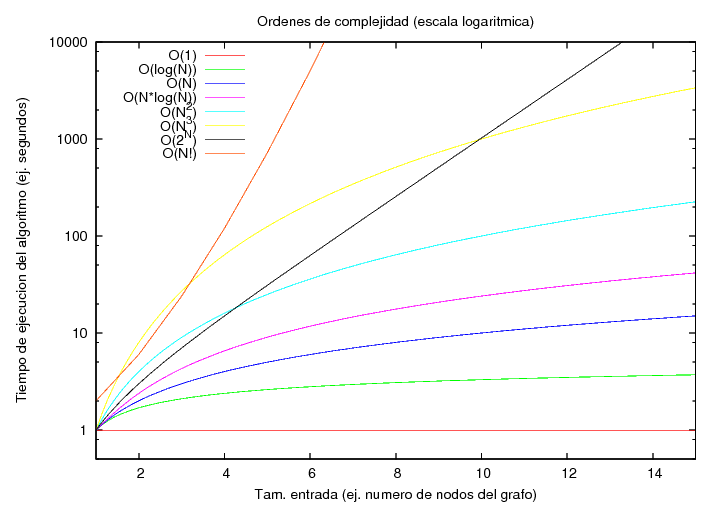
\includegraphics[scale=0.6]{imagenes/5}
	\caption{Grafico con las curvas de los ordenes de complejidad en una escala logaritmica}
	\label{ordenes}
\end{figure}

En la figura \ref{ordenes} se pueden ver los tiempos que demora en procesar un algoritmo una cantidad de datos determinada en una escala logar�tmica donde mientras m�s arriba diverge la funci�n m�s dif�cil o m�s tiempo toma su calculo. En computaci�n se tienen distintos tipos de clases de complejidad para clasificar los problemas seg�n la mejor soluci�n descubierta por el momento siendo las mas conocidas la clase P, los problemas que pueden ser resueltos en tiempo polinomial, y NP, los problemas que pueden ser resueltos en tiempo polinomial pero solo por una maquina no determinista. Estos �ltimos poseen un subconjunto de problemas conocidos con una complejidad mucho mayor y que son reducibles entre ellos, es decir, un problema puede ser representado o transformado a una variante equivalente de otro problema dentro de ese subconjunto.

Otra unidad de medida diferente al tiempo es la unidad de espacio. Con esto se eval�a la cantidad de memoria necesaria que requiere una soluci�n. En esta tesis se tendr� �nfasis en la unidad de tiempo pero en la secci�n ``Validaci�n'' se mencionar� brevemente los cuidados que hay que tener con el espacio.


\section{Teor�a de Grafos}

Un campo que ha tomado gran importancia en la computaci�n es la teor�a de grafos. Los grafos son una estructura que esta compuesta por dos elementos: los nodos y las aristas. Las aristas pueden tener direcci�n y en ese caso se habla de un grafo dirigido.

\begin{figure}[!h]
	\centering
	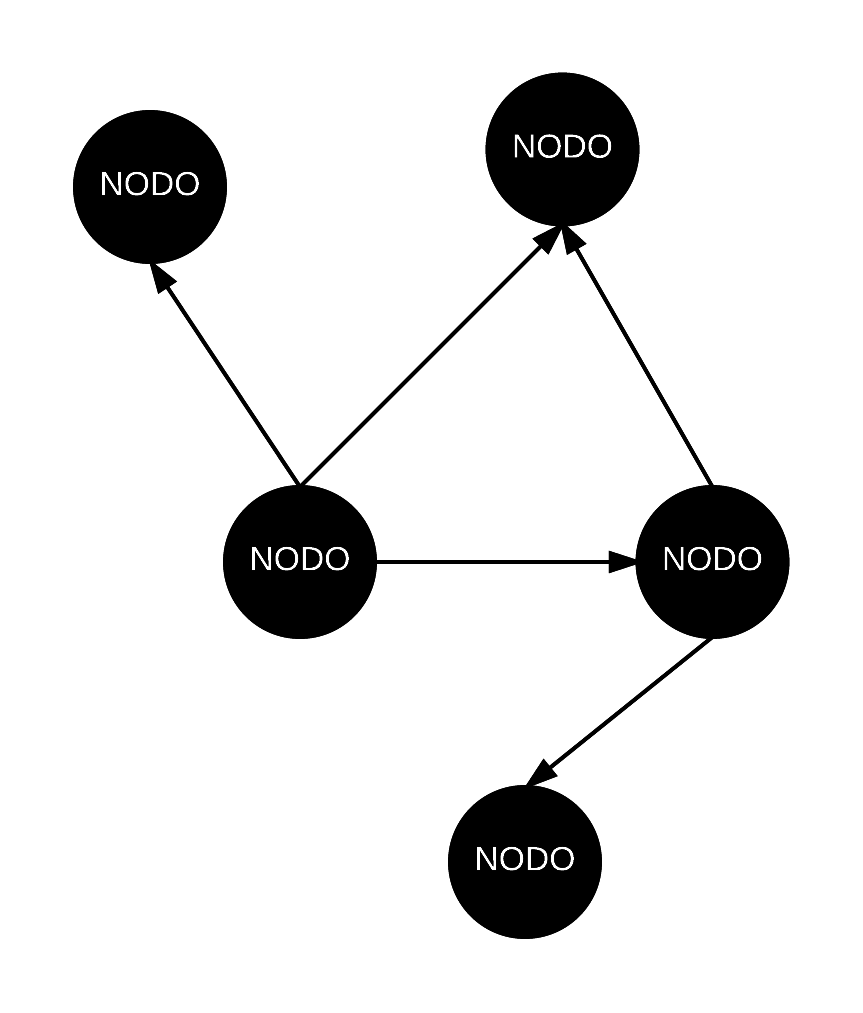
\includegraphics[scale=0.9]{imagenes/6}
	\caption{Ejemplo de grafo dirigido}
	\label{directed_graph}
\end{figure}

La forma que posee esta estructura ha sido de utilidad debido a que muchas cosas pueden representarse mediante ella. Por ejemplo, posiciones dentro de un mapa pueden ser representadas por nodos y las aristas son los caminos entre ellas teniendo la habilidad de agregar valores (la arista tiene un valor mayor mientras mas alejados est�n los nodos). A partir de esto y una representaci�n matem�tica de los elementos de un grafo pueden resolverse problemas te�ricos con variada utilidad en la practica. Siguiendo el mismo ejemplo anterior, la soluci�n te�rica del camino con aristas de menor valor entre dos nodos podr�a representar el camino mas corto entre dos lugares geogr�ficos.

Existen variados tipos de grafos entre ellos los grafos conexos que se definen como los grafos donde para todo par de nodos se tiene un camino que los une. Cuando no se posee un grafo totalmente conexo se pueden tener subconjuntos que si lo sean a los que llamaremos componentes conexas.

\textbf{imagen de grafo conexo y de componentes conexas}

Otro caso particular de grafo son los arboles. Este es un grafo conexo en que la uni�n de todo par de v�rtices es �nica, es decir, se posee solo un camino entre un nodo y otro. En este caso, si bien las aristas en un �rbol no poseen direcci�n, se puede armar un estilo de jerarqu�a donde el nodo desde donde se originan las primeras aristas es conocido como la ra�z. Adem�s, es com�n en este tipo de estructuras describir los nodos como padres e hijos de acuerdo al nivel que poseen y desde cual nodo se originan. Los nodos que ya no poseen nodos hijos son conocidos como las hojas del �rbol.

Dentro de la teor�a de grafos y las componentes conexas, existe un concepto �til de comprender para esta memoria conocido como ``la componente gigante'' (Giant component en ingles). Si bien es un estudio que implica variadas cosas y utiliza conceptos de probabilidades, uno de los elementos importantes es que si se posee un grafo de $n$ nodos y se van adicionando aristas aleatorias, si la cantidad de aristas adicionadas supera aproximadamente $n/2$ con alta probabilidad se tendr� una componente conexa gigante. \textbf{Quizas no sea tan importante en la memoria y deba sacarse}


\section{Optimizaci�n Combinatorial}

La optimizaci�n es un �rea de las matem�ticas donde se busca determinar la mejor manera de realizar una actividad bajo criterios extra�dos del modelamiento del problema.  Un ejemplo es maximizar los ingresos de alguna instituci�n o disminuir los tiempos de ejecuci�n de una tarea.

En el caso particular, la optimizaci�n combinatorial involucra encontrar la soluci�n dentro de un conjunto discreto. Com�nmente, en los problemas relacionados se tiene la opci�n de encontrar la soluci�n con una b�squeda exhaustiva pero debido a la magnitud del conjunto el tiempo necesario para llegar a la confirmaci�n de que se esta en presencia de la mejor soluci�n se vuelve muy grande y por lo tanto el m�todo no es factible.

Usualmente, un problema de optimizaci�n combinatorial puede representarse como un �rbol de decisi�n. Es decir, un grafo donde cada nodo diverge hacia otros nodos seg�n la cantidad de opciones que se tiene sobre una variable, de esta manera para cada variable que se debe definir se tendr� una representaci�n visual de alguna elecci�n. Ejemplificando, si tenemos un problema de dos preguntas que se pueden responder con si o no, tendremos un nodo donde se decida sobre la primera pregunta y se tendr� dos aristas debido a las dos opciones de respuesta. Luego, en los nodos hijos se representara la decisi�n de la segunda pregunta pero teniendo como dependencia la decisi�n ya tomada, por lo tanto las hojas de este �rbol de decisi�n representan las distintas combinaciones que se pueden obtener del problema conjunto.

\textbf{imagen con un arbol de decision peque�o}

Variados problemas de optimizaci�n combinatorial presentan una complejidad de clase NP y muchos de ellos pueden ser representados con grafos. Adem�s, como no se logra encontrar una soluci�n r�pida, los problemas son estudiados en profundidad document�ndose distintos avances con algoritmos y heur�sticas. Estos pueden tener mejoras en casos particulares y es importante conocer algunos de ellos que se parezcan al caso de la presente memoria.

Casos conocidos son el problema de la mochila o el de mudanza. En ellos es necesario poner objetos dentro de alg�n contenedor de tal manera de maximizar la cantidad de objetos que se pueden llevar, maximizar la utilidad de esos objetos, minimizar la cantidad de contenedores necesarios u otra optimizaci�n. Martello y Toth \cite{bib3,bib4} propusieron algoritmos para resolver este tipo de problemas siendo una de ellos la estrategia de ramificaci�n donde el ordenamiento de los objetos se realiza por valor decreciente (tama�o, peso o importancia dependiendo del objetivo). De esta manera, para cada nodo de decisi�n se tiene el objeto de mayor valor y es ubicado en el contenedor de la m�s pr�xima factibilidad.

Cuando no se posee una soluci�n exacta adecuada se puede incurrir en reducciones del conjunto de combinaciones con relajaciones de las restricciones. Aun as� se debe tener presente conceptos como el de programaci�n din�mica para no incurrir en c�lculos reiterados de un subconjunto. Para ejemplificar lo anterior podemos intentar resolver la sucesi�n de fibonacci la cual esta dada por:

$$F(n) = F(n-1) + F(n-2) , F(0) = 0, F(1) = 1$$

Para calcular el valor de $F(5)$, de acuerdo a la secuencia, se debe calcular el valor de $F(4)$ y $F(3)$. Aun as�, para calcular el valor de $F(4)$ se debe calcular nuevamente el valor de $F(3)$ y el valor de $F(2)$. Si se siguiera el orden anterior y fuese efectuado por un computador, el calculo de $F(3)$ se realizar�a repetitivamente siendo que no es necesario si ya fue calculado una vez, por lo que se podr�an realizar dos mejoras a la forma en que fue orientada la soluci�n del problema: tener en memoria los c�lculos ya hechos para consultarlos posteriormente o seguir una estrategia bottom up (comenzar desde $F(1)$ hasta llegar a $F(n)$).

\begin{figure}[!h]
	\centering
	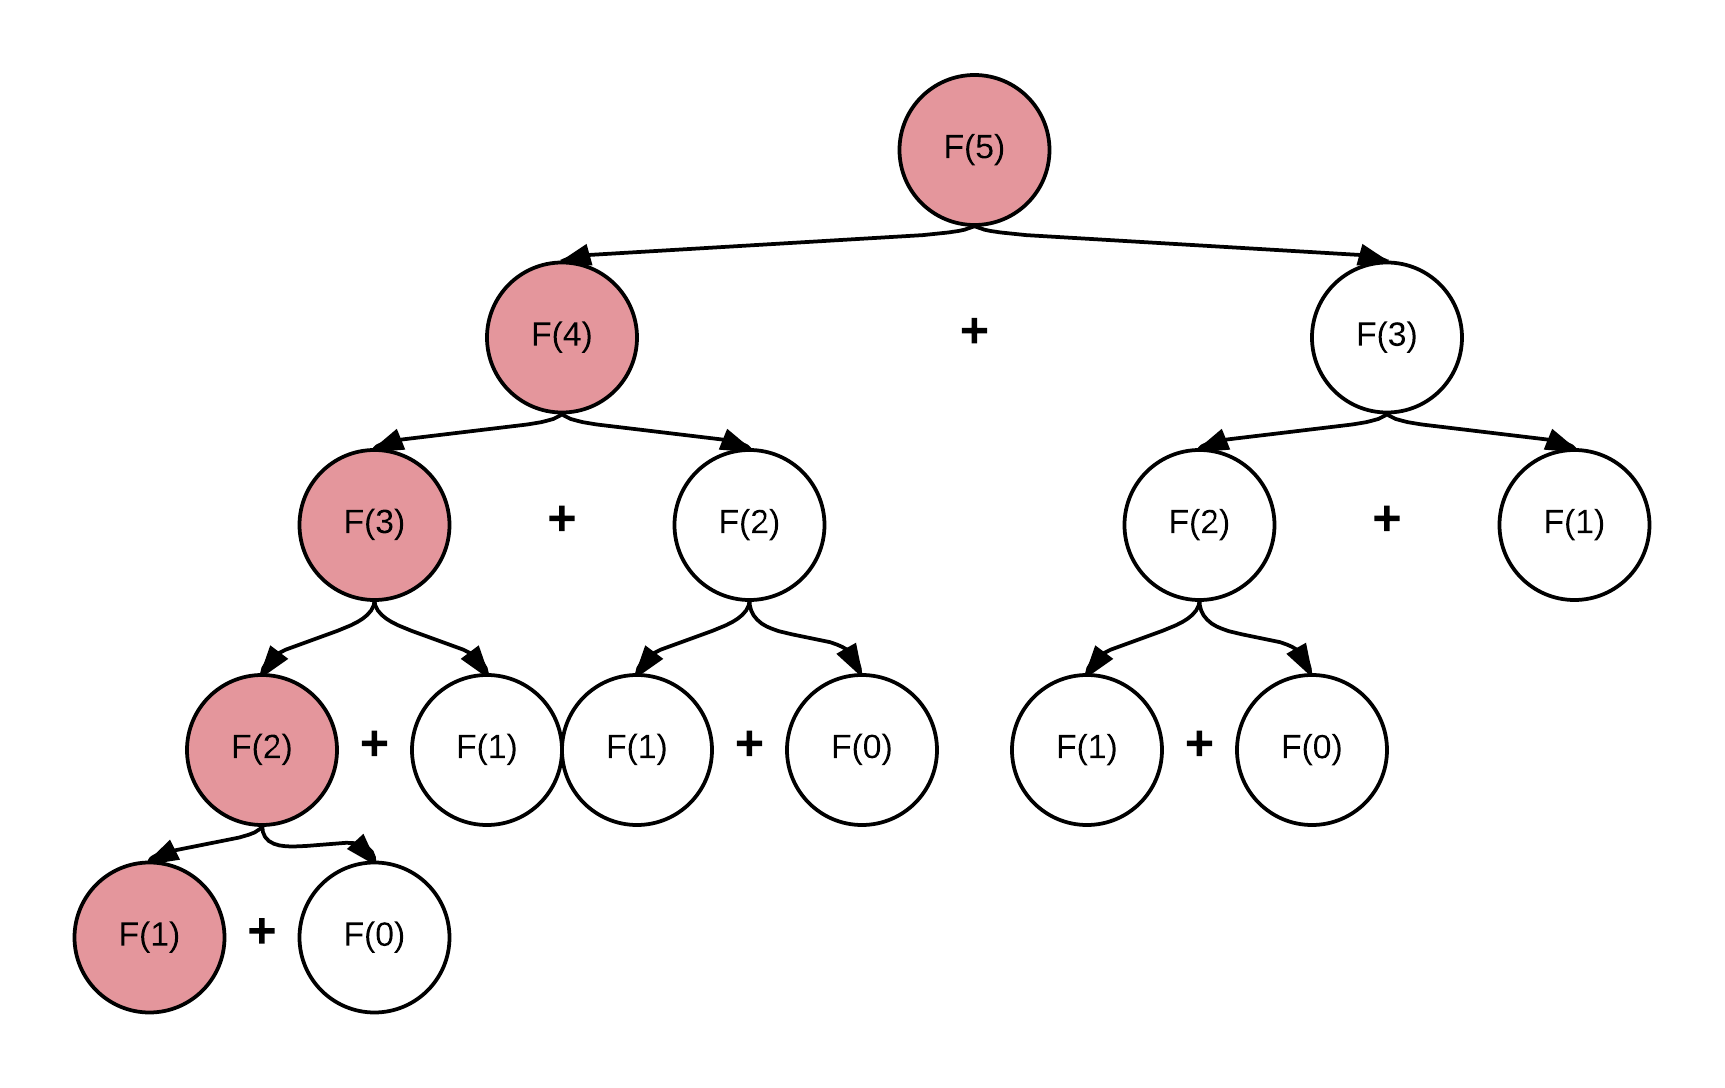
\includegraphics[scale=1]{imagenes/7}
	\caption{Calculos hechos en serie de fibonacci siguiendo perspectiva top-down.}
	\label{fibonacci}
\end{figure}

 % Marco Teorico
\chapter{El Problema: Situacion Actual}

El recuento de cr�ditos inicialmente era un proceso netamente manual. Estaba constituido por un solo actor que a partir de la experiencia pod�a manejar las diferentes condiciones que se generaban. Ante eventualidades, como casos extra�os en el que faltaban UD�s en cierto plan, el mismo actor tenia la potestad de flexibilizar las reglas para chequear si realmente un alumno cumpl�a con la carrera.

Como se mencion� en la descripci�n del proyecto, este proceso fue mejorando poco a poco logrando que existieran componentes autom�ticas en el procedimiento, tratando de suplir todo el conocimiento generado del actor mencionado en el p�rrafo anterior. Aun as�, la parte automatizada posee errores de tal manera que se debe realizar un chequeo manual posterior.

Los errores se deben a la complejidad de las reglas que se deben cumplir y a la naturaleza del problema. Por ende, se ahondar� en ello en la secci�n �Combinaciones� explicando el modelo e implementaci�n actual.

Finalmente, en la secci�n del proceso actual se abordar� el procedimiento realizado por el SGD para suplir la falta de certeza de la heur�stica en ciertos casos y las estad�sticas de ocurrencia de los errores.


\section{Combinaciones}

Para entender el problema de forma mas detallada podemos realizar un simplificaci�n del recuento y reducirlo a un problema de mudanza (bin packing). Para ello debemos asimilar los planes como si fueran cajas, y los ramos como si fueran elementos que deben ser guardados dentro de estas cajas para poder ser trasladados.

Para este problema la soluci�n trivial seria ir intentando distintas combinaciones posibles de tal manera de lograr que todos los elementos sean guardados. Esto seria la soluci�n a fuerza bruta del problema entregando la mejor soluci�n pero el tiempo necesario para realizar todas combinaciones posibles es muy grande. No se posee un tiempo ilimitado y, por ende, lo mas natural ser�a comenzar a privilegiar algunos elementos guardando inicialmente los de mayor valor para luego ir rellenando con los de menor valor o los que se podr�an dejar olvidados (Como lo realizado por Martello y Toth descrito en el �Marco Teorico").

En el caso de la soluci�n presente del recuento de UD�s se utiliza la anterior heuristica. Se consideran los ramos de valor aquellos que poseen mayor nota y son de nivel mas alto (se debe privilegiar poner los ramos de mejor nota en la carrera debido a que ellos son considerados para el promedio final). Finalmente, esto ir�a mediante backtracking visitando todas las soluciones posibles pero teniendo en un inicio ramos de importancia fijos.

Matem�ticamente, se puede definir que un ramo $r$ puede pertenecer a cierto conjunto de planes $P_r$ de tama�o $n_r$, y que un plan se ve cubierto si y solo si tiene asignado una cantidad determinada de ramos mayor o igual a $L_p$. Por lo anterior, el determinar el cumplimiento del plan y la nota se trata de un problema de asignaci�n en el que se puede usar el ramo en alguno de sus planes. Si consideramos $X_{rp} \in \{0,1\}$ como la variable de decisi�n que determina si se usa el ramo $r$ en el plan $p$, el modelamiento del problema de calcular si se cumple el plan quedar�a determinado por:

$$ max \sum_{r}^{Ramos} \sum_{p}^{Planes} X_{rp} $$
$$ s.a.\ \ \ \sum_{r}^{Ramos} X_{rp} > L_{p} \ \ \ \ \forall p \in planes $$
$$ \sum_{p}^{P_{r}} X_{rp} \leq 1 \ \ \wedge \sum_{p}^{planes \setminus P_{r}} X_{rp} \leq 0 \ \ \ \ \forall r \in ramos $$

De esta forma, el orden de complejidad de este modelo vendr�a dado por la pitatoria $ \prod_{r} n_{r} $. Es decir, en el caso hipotetico en que $m$ ramos tuvieran tres opciones donde ser ubicados se tendr�a $ \prod_{r} 3 \Rightarrow O(3^m)$, lo que equivale a un orden de complejidad exponencial. A partir de esto se descarta, a priori, la posibilidad de un problema mucho mayor en que al ser combinaciones de todos los ramos contra todos los planes se obtendr�a un orden factorial de complejidad. 

Como se posee poco tiempo en un sitio web, este modulo es detenido a los quince segundos y por lo tanto puede suceder que hasta ese tiempo no se haya visitado una combinaci�n que diga que todos los planes se cumplen siendo que quiz�s mas adelante podr�a encontrarla. En el caso del calculo de la nota se sigue el mismo comportamiento debido a que se realiza en conjunto con la comprobaci�n del cumplimiento del plan principal. 

Si bien se asegura que se tiene una buena distribuci�n porque se asignaron los ramos de importancia, no se tiene certeza de la correctitud en el punto donde es detenido el algoritmo. Aun as�, se privilegi� este procedimiento porque estos casos generan un falso negativo, es decir, el error que puede producir es que un alumno que puede titularse el sistema le diga que aun no puede. Para estos sucesos se siguen los pasos que se explicaran en la secci�n de �proceso presente�.  

Aun as�, lo descrito anteriormente solo es una relajaci�n del problema. Si se consideran todas las reglas especificas de cada plan se puede armar un modelo como sigue:

$$ max\ \ usar_{carr,carr} \ \ :\ carr \in planes $$
$$ s.a. \sum_{p}^{planes} usar_{op} \leq 1 \ \ \ \forall o \in objetos \setminus o \neq p $$
$$ usar_{pp} \leq usar_{op} \ \ \ \forall p \in planes, \forall o \in objetos\ \setminus\ regla_{p} = todo \wedge pertenece_{op} = 1 $$
$$ usar_{pp} \cdot cantidad_{p} \leq contar_{p} \ \ \ \forall p \in planes\ \setminus\ regla_{p} = contar $$
$$ usar_{pp} \cdot cantidad_{p} \leq uds_{p} \ \ \ \forall p \in planes\ \setminus\ regla_{p} = ud $$
$$ usar_{pq} \leq contar_{p} \ \ \ \forall p,q \in planes\ \setminus\ regla_{p} = contar \wedge pertenece_{pq} = 1 $$
$$ usar_{pq} \leq uds_{p} \ \ \ \forall p,q \in planes\ \setminus\ regla_{p} = ud \wedge pertenece_{pq}=1 $$
$$ usar_{pq} \leq usar_{pp} \ \ \ \forall p,q \in planes\ \setminus\ regla_{p} = todo \wedge pertenece_{pq}=1 $$

En este modelo se generaliza lo que son los ramos y los planes debido a que se comportan de manera parecida. Es decir, como un plan puede poseer tanto ramos como subplanes y adem�s un ramo puede verse como un plan debido a que puede poseer equivalencias, finalmente pueden modelarse como un �nico conjunto llamado objetos ($ramos \cup planes$). Adem�s, puede utilizarse una variable que en el modelo le llamamos ``Usar'' que implica que un elemento ``i'' esta siendo usado en un elemento ``j'' de tal manera que esto implica los objetos considerados dentro de un plan. Un objeto estar�a siendo usado en si mismo si y solo si es un ramo aprobado o es un plan donde se cubren todas las reglas relativas a �l, y por ende de esta manera se podr�a verificar cuando una carrera se cumple.

De esta manera las restricciones vendr�an a explicar reglas parecidas al modelo simplificado como que un objeto puede ser usado una �nica ocasi�n, que cuando se tiene una regla �todo" se deben usar todos los elementos dentro de �l y que cuando se tiene regla �contar� o �uds� se debe utilizar una cantidad mayor o igual a la determinada. 

La forma que esta implementado actualmente el sistema es mediante backtracking. Es decir, lo que se realiza es tomar un ramo de una lista, fijar el plan donde puede ser utilizado (escogiendo el primero de los candidatos para ese ramo) y continuar con el ramo siguiente. En cada paso se va evaluando si la soluci�n que se tiene en ese instante es mejor que una guardada en una variable global y si lo fuese se actualiza esa variable. Luego, cuando todos los ramos se asignaron, el algoritmo debe ir devolvi�ndose de manera tal de ir probando los siguientes candidatos de cada ramo pero volviendo a calcular las combinaciones de los ramos siguientes porque cambi� la situaci�n. 

Ejemplificando, si se poseen tres ramos A, B y C, se deben asignar los dos primeros y calcular todas las opciones para C. Luego, se debe retroceder un paso, cambiar el candidato de B y volver a calcular las opciones de C. Asi de manera sucesiva hasta lograr calcular todas las opciones de B y A, respectivamente. Como se dijo anteriormente, no se posee un tiempo infinito y, por ende, el algoritmo debe detenerse, por lo tanto es probable que no se logre retroceder hasta A y solo se quede con el calculo de las mejores opciones de B y C. Es por ello que los ramos determinados en un principio deben asignarse de la mejor manera posible para que el costo de dejar el algoritmo inconcluso se minimice.


\section{Proceso Presente}

Inicialmente, gran parte del recuento de UD�s pertenec�a a �Secretaria de Estudios� ya que ellos verificaban el cumplimiento de los requisitos acad�micos del proceso de titulaci�n. Aun as�, por la complejidad del proceso y las fallas encontradas en el modulo autom�tico la Subdirecci�n de Gesti�n Docente (SGD) debi� ser parte del proceso para generar una propuesta inicial.

Este proceso inicia con la aprobaci�n de un ramo terminal. Es decir, al cumplir un ramo que esta cercano al termino de la carrera se puede confirmar que un alumno va necesitar la comprobaci�n de sus antecedentes acad�micos. Inicialmente, eso si, es necesario procesar la licenciatura asociada a la carrera del alumno para proseguir normalmente.

Luego, el SGD valida el resultado entregado por el modulo del recuento de UD�s verificando que no se este en presencia de un falso negativo. Esto se evidencia ya que el sistema menciona que el alumno no cumple el plan y existen ramos no usados que con un re-ordenamiento de los ramos utilizados pueden disponerse y lograr una combinaci�n v�lida.

La b�squeda de una combinaci�n puede ser lenta y por ello se pueden recibir notificaciones de parte del alumno que busca que su proceso contin�e como es debido. Adem�s, �l posee mucho mayor conocimiento de su avance curricular y por ende puede ayudar a la b�squeda de la soluci�n. Dado esto, existe un modulo en U-Campus que permite la interacci�n entre alumnos e integrantes del SGD.

\begin{figure}[!h]
	\centering
	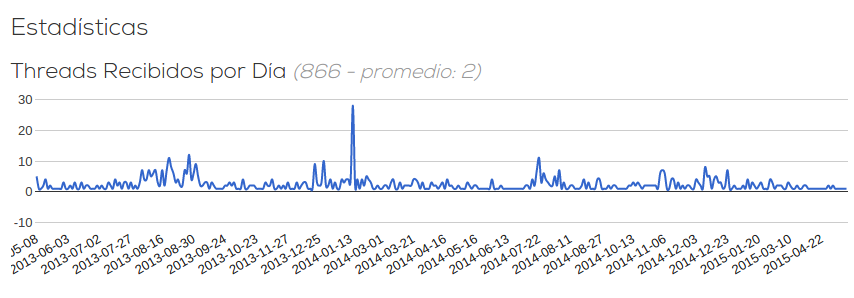
\includegraphics[scale=0.55]{imagenes/8}
	\caption{Estadisticas de peticiones por dia relacionadas al recuento de UD's.}
	\label{estadisticas_sgd}
\end{figure}

Se posee un promedio de dos consultas por dia relacionadas con el recuento. Estas son resueltas com�nmente en algunos d�as pero existen ocasiones en que toman mayor tiempo (meses) debido a que involucran normas adicionadas en los cambios de planes de estudios. Esto esta �ntimamente relacionado con las versiones de los planes explicadas en la descripci�n del proyecto.

Finalmente, cuando ya se posee una combinaci�n valida o cuando el alumno aprueba lo necesario para el cumplimiento del plan, se env�a el resultado del sistema con observaciones de los cambios necesarios para obtener la combinaci�n valida si se requiere. Esta es recibida por la Secretaria de Estudios quien valida la propuesta donde la acepta confirmando el cumplimiento de los requisitos acad�micos o la rechaza para que el SGD justifique de mejor manera las observaciones agregadas.

Otros de los procesos que tiene a cargo el SGD son la inscripci�n acad�mica, el catalogo de cursos, el calendario acad�mico, entre otros. Muchos de ellos presentan alta carga y con tasas de errores dependientes del tiempo involucrado en ellos para una correcta planificaci�n. Si se posee una mejora en la certeza del recuento de UD�s se disminuir�an los reclamos por parte del alumnado y la cantidad de rechazos por parte de Secretaria de Estudios.



 % El Problema: Situacion actual
\chapter{Soluci�n: Modelo y Redise�o}

Dentro de las opciones mencionadas en un problema de optimizaci�n combinatorial se encuentra la reducci�n del espacio de soluciones. Es decir, un buen entendimiento y modelamiento del problema deber�an implicar un espacio m�nimo pero no necesariamente, y es por ello que pueden existir aun formas de abordar de esta manera el redise�o.

En un recuento de UD's un alumno que esta cercano a titularse posee aproximadamente 70 ramos. Un plan de titulo profesional posee alrededor de 18 subplanes los cuales poseen distintas reglas y por ende los ramos antes descritos pueden utilizarse o no, dependiendo estas normas. Aun as�, pensando en la flexibilizaci�n inicial que se hizo en la secci�n ``Problema'', si los ramos poseen en promedio tres lugares donde ser ocupados tendr�amos un numero cercano a $3^{70}$ combinaciones que recorrer para decidir cual seria la soluci�n correcta. Si se eliminara un ramo se tendr�a tres veces menos combinaciones.

\begin{figure}[!h]
	\centering
	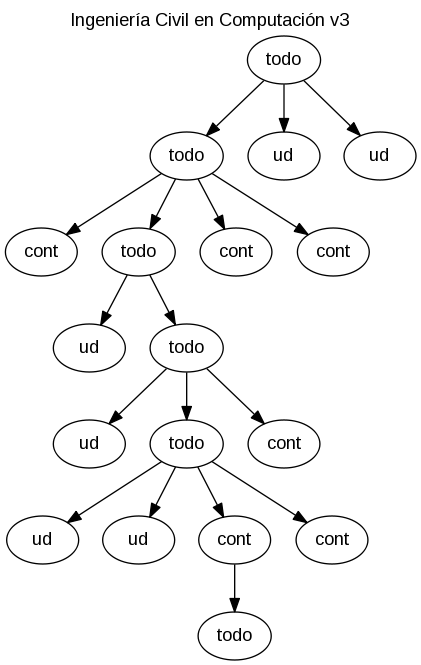
\includegraphics[scale=0.4]{imagenes/9}
	\caption{�rbol de planes con sus respectivas reglas como etiqueta de los nodos.}
	\label{arbol_reglas}
\end{figure}

En la imagen \ref{arbol_reglas} se observan las reglas de los planes de la tercera versi�n de la carrera de ingenier�a civil en computaci�n. Han sidos dispuestos como un �rbol de acuerdo a la dependencia que tienen entre ellos ya que, recordando, un plan puede tener subplanes dentro de �l. Si desde la ra�z del �rbol se va bajando de nivel se puede observar que se sigue una linea donde la regla de los planes es ``todo'', es decir, se deben cumplir obligatoriamente todos los elementos pertenecientes a esa linea. Por ende, todos los ramos que se encuentran dentro de esos planes podr�an verificarse en un inicio reduciendo la cantidad de ramos que pasar�an posteriormente por el algoritmo.

Si bien se puede pensar que esta es una reducci�n considerable ya que se puede sacar del calculo cerca del $50\%$ de los ramos, de todas formas no es del todo significativa ya que com�nmente estos ramos son considerados obligatorios dentro del modelamiento de los planes y por ende poseen a lo mas dos lugares donde ser ocupados. Adem�s, se debe tener precauci�n debido a que, por ejemplo, los ramos dentro del plan de regla ``todo'' que esta en el nivel inferior poseen un plan padre que tiene regla ``contar'' y podr�a cumplirse sin la necesidad de aprobar los ramos del subplan.

Siguiendo la misma linea pueden reducirse los ramos que poseen un lugar donde ser ocupados debido a que si se agregaran al procesamiento del algoritmo, este considerar� que pueden ocuparse o dejarse fuera del calculo, y por ende no se estar�a en presencia de tan solo un lugar donde ser ocupado, si no que dos. Eso s� existe un diferencia entre este tipo de ramos que con los con planes con regla ``todo'', ya que estos realmente podr�an no ocuparse. Aun as�, esta reducci�n podr�a considerarse dentro de las opciones porque para aprobar una carrera se podr�a ocupar la m�xima cantidad de ramos posibles siendo perjudicada la nota pero se realizar�a un post-procesamiento para mejorar aquello.

Lamentablemente la implementaci�n actual ya realiza una reducci�n descartando poner un ramo dentro de un plan si este ya esta cubierto. Si se realizar� la reducci�n del p�rrafo anterior, se agregar�an ramos con menor nota y el orden de poner los ramos de mejor nota inicialmente se ver�a entorpecido, provocando que la reducci�n de la implementaci�n actual funcione incorrectamente. De todas formas se implementaran ambas y se realizar� una comparaci�n para decidir cual es mejor dentro de ellas pero, a priori, debido a que los ramos reducidos de la implementaci�n actual pueden tener mas que una opci�n donde ser ubicados, implicar�a una reducci�n mayor y ser�a una mejor decisi�n.

Yendo a la b�squeda de mejora dentro de la heuristica ya implementada, se debe encontrar una perspectiva distinta para ver el problema. Si se modela �ste como un grafo podr�amos encontrar formas dentro de la teor�a que podr�an servir como mejora. Por ende, si se consideran los ramos como si fueran nodos unidos solo si poseen un plan en com�n dentro de sus opciones, se tendr�a una imagen como la de la figura \ref{grafo_general}.

\begin{figure}[!h]
	\centering
	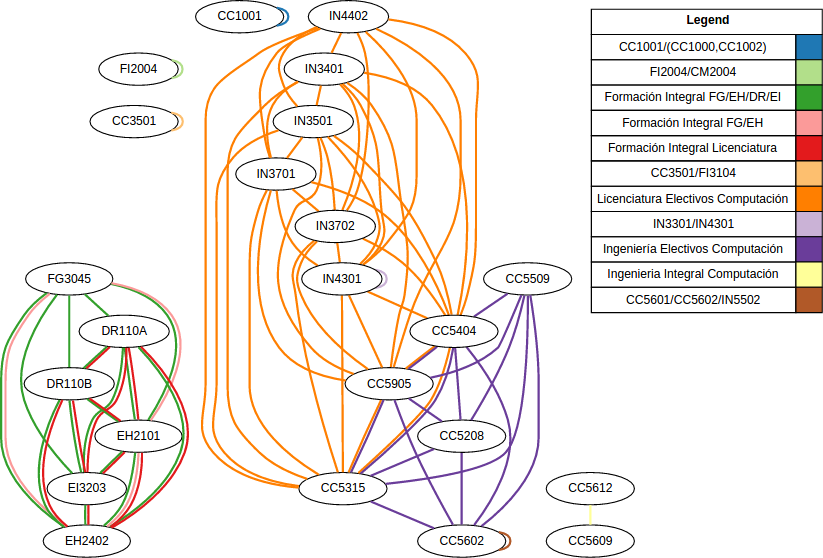
\includegraphics[scale=0.5]{imagenes/10}
	\caption{Conversi�n del problema en un grafo}
	\label{grafo_general}
\end{figure}

Se observa un grupo de ramos de un alumno de la carrera de ingenier�a civil en computaci�n, en donde el nodo posee el nombre del ramo en su interior y entre ellos est�n unidos por aristas de distintos colores. El color indica el plan por el cual est�n unidos (detallado en la leyenda) existiendo ramos donde se origina un solo color debido a que solo tienen un candidato donde ser ubicados y pueden no estar asociados a ning�n otro nodo.

Adem�s, como se observa, existen componentes conexas dentro del grafo. Si bien esto a priori puede no significar mucho, si se contrasta con la implementaci�n actual toma sentido un tipo de mejora hablada anteriormente como lo es la programaci�n din�mica. Si se toma un ramo A y se puede gastar en los planes P o Q, sea cual sea la decisi�n con ese ramo esto no va a afectar la decisi�n de un ramo B que se puede gastar en los planes R o S. Esto debido a que no comparten ning�n plan y pueden tomarse como problemas independientes. Se volver�an dependientes uno sobre el otro si se tuviera un ramo C que pueda gastarse en Q o R (ambas opciones de A y B) debido a que si se gasta en Q implicar�a menos espacio para A o si se gasta en R significar�a menos espacio de soluci�n para B. La soluci�n actual esta considerando todos los ramos y sus decisiones dependientes de los dem�s siendo que lo que significan las componentes conexas dentro del grafo es que existen subproblemas independientes.

De todas manera, inicialmente se consider� una dependencia completa debido a la forma de �rbol de dependencia de los planes. Por lo mismo, se debe aun considerar reglas que no est�n siendo visualizadas dentro del grafo pero se ven en la visualizaci�n de reglas (figura \ref{arbol_reglas}) como lo son la posibilidad de no cumplir un plan debido a que el plan padre se cumple. 

\begin{figure}[!h]
	\centering
	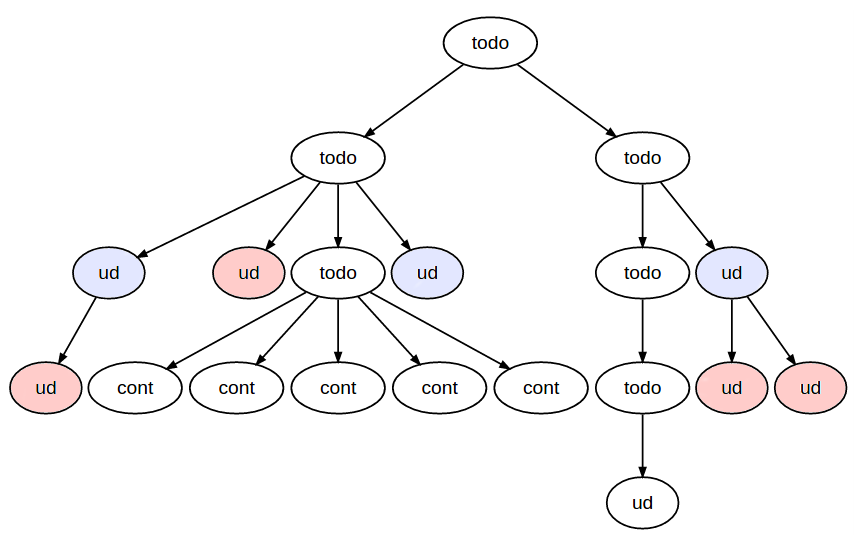
\includegraphics[scale=0.4]{imagenes/11}
	\caption{�rbol de reglas para la carrera Ingenier�a Civil Electricista (v2).}
	\label{arbol_reglas_electrica}
\end{figure}

En el caso de la imagen \ref{arbol_reglas_electrica}, dado el calculo de un grafo de ramos de la segunda versi�n de la carrera ingenier�a civil electricista se pintaron en el arbol de reglas de los planes dos componentes conexas (azul y rojo). Si se sigue el razonamiento de uno de los p�rrafos anteriores los arboles de decisi�n de estas componentes conexas deber�an estar separados pero dado que un plan no necesariamente debe cumplirse ya que puede cumplirse el padre estas deber�an estar juntas. Podemos aprobar los planes azules y solo un plan rojo (el que no tiene un padre azul) y estar�amos cumpliendo todas las reglas pero si lo consideramos problemas independientes en la componente conexa roja se har� esfuerzo por completar los planes de nivel bajo aunque no sea necesario.

Teniendo todas estas cosas en consideraci�n se lograr�a reducir el problema en varios problemas peque�os. Si anteriormente se ten�an $3^{30}$ combinaciones, con esta mejora se lograr�a una reducci�n a problemas independientes y el calculo se har�a con sumas, es decir, si se pudiera dividir en tres componentes conexas con diez ramos cada uno se tendr�a la adici�n $3^{10}+3^{10}+3^{10}$ lo que es igual a $3^{11}$ combinaciones.

\begin{figure}[!h]
	\centering
	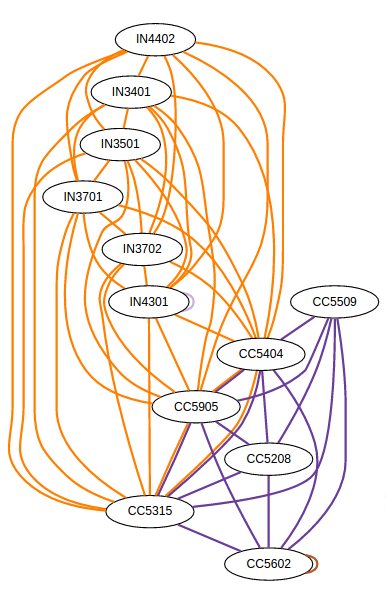
\includegraphics[scale=0.5]{imagenes/12}
	\caption{Extracto de la figura \ref{grafo_general} para evidencia la recursividad de las componentes}
	\label{grafo_reducido}
\end{figure}

Si se vuelve a ver la imagen donde esta el grafo con las componentes conexas (figuras \ref{grafo_general} y \ref{grafo_reducido}), se puede ver que la componente con mayor cantidad de ramos posee aristas de color naranjo y morado. Los ramos que est�n uniendo estos dos colores son tres (CC5315, CC5905 y CC5404) y si se toma inicialmente la decisi�n sobre ellos podr�an formarse dos componentes conexas separadas. Es decir, decidir sobre un ramo podr�a formar nuevas componentes reduciendo aun m�s el espacio de soluciones. Aun as�, el calculo de qu� ramos tendr�an mayor probabilidad de ocasionar esta separaci�n y el ordenamiento seg�n ello podr�a significar un coste mayor debido a que se estar�a rompiendo el orden inicial de mayor valor (al igual que una de las reducciones que se pens�). Por lo tanto, se puede implementar el calculo recursivo de componentes conexas y evaluar los dos posibles ordenamientos para ver cual ocasiona una reducci�n mayor.

Finalmente, una mejora final considerada en esta memoria es el cache. Este consiste en poseer parcialmente en memoria elementos, de manera que sea m�s facil obtenerlos desde esta memoria que ser calculados o extraidos de otro lugar. Si bien con el calculo de componentes conexas se estar�a eliminando gran parte de los elementos repetidos, tambi�n pueden existir c�lculos repetidos por la formaci�n de nuevas componentes conexas que ya se hab�an formado anteriormente las cuales pueden guardarse en memoria cache para no realizar su calculo nuevamente.

Si se tuviera un ramo que al asignarse genera tres componentes conexas, el ramo podr�a haberse asignado dentro de esas tres opciones solamente. Si evaluamos paso a paso como se comportar�a el algoritmo al asignar este ramo podremos evidenciar el calculo repetido.

\begin{figure}[!h]
	\centering
	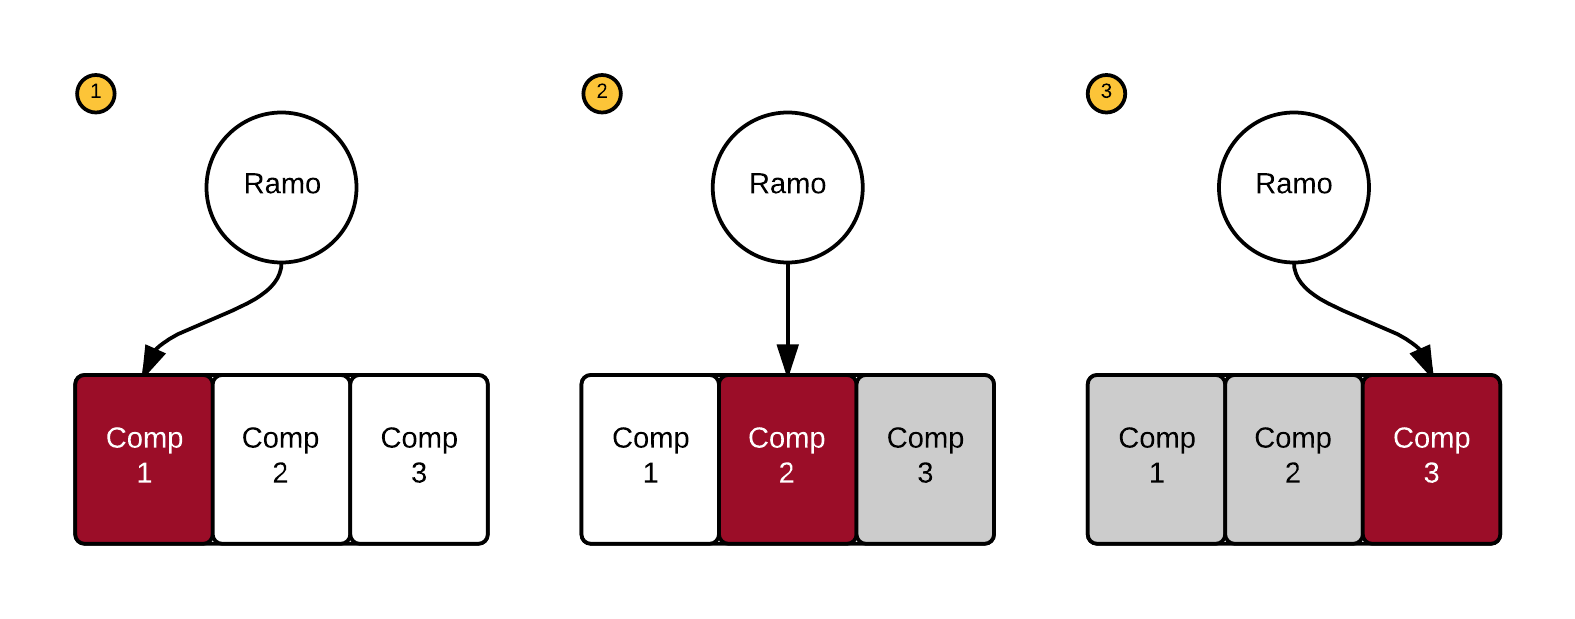
\includegraphics[scale=0.9]{imagenes/13}
	\caption{Comportamiento del cache. En rojo el lugar donde se ubica el ramo y en blanco la componente donde no se posee. En gris los calculos que pueden ser obtenidos desde la memoria cache ya que ya fueron calculados anteriormente.}
	\label{cache}
\end{figure}


Al inicio, el ramo ser� asignado en la primera componente calcul�ndola considerando el ramo dentro de su soluci�n. En cambio las otras dos componentes se calcularan sin considerar el ramo. Una vez hechos esos c�lculos, el algoritmo debe devolverse y calcular que pasar�a si el ramo fuera asignado en la segunda componente conexa. All�, la segunda componente tendr� probablemente una soluci�n distinta porque en esta ocasi�n debe considerar el ramo, la primera componente tambi�n deber� hacer su calculo nuevamente porque ahora no debe considerar el ramo (anteriormente si lo hab�a hecho) pero la tercera componente volver� a calcularse sin considerar el ramo lo que podr�a guardarse dentro de un cache y no necesitar calcularla.

Lo anterior, debido al calculo del algoritmo, solo se producir�a con ramos que generan mas de dos componentes conexas lo que es de baja probabilidad. Aun as� se implementara dentro de esta memoria porque puede significar mejoras considerables si la componente conexa guardada fuese de un volumen grande.



 % Soluci�n: Modelo y Redise�o
\chapter{Implementaci�n}

A continuaci�n se mencionar�n los pasos seguidos en la implementaci�n. Estos ser�n explicados de forma concisa sin entrar en detalles de programaci�n para un entendimiento m�s bien superficial de lo t�cnico, manteniendo una mirada global del cumplimiento del dise�o y el modelo. De todas formas, en el primer ap�ndice se deja a disposici�n parte del c�digo implementado para evidenciar detalles de la puesta en funcionamiento.

Para la implementaci�n se utiliz� como base lo hecho en las versiones pasadas del recuento de unidades docentes. En �stas el recuento se divid�a en cuatro funciones importantes destacando dos de ellas: la inicial y la recursiva. La funci�n inicial realiza la petici�n de los ramos y planes a partir del rut y carrera de un alumno, limpia estos datos, realiza asociaciones como las relaciones entre ramos de distintas versiones, llama a la funci�n recursiva y, finalmente, retorna los resultados. Por otra parte, la recursiva realiza todo el procesamiento de la heur�stica anteriormente descrita llam�ndose a s� misma por cada asignaci�n de ramo. Adem�s, debe convocar a las otras dos funciones donde se propaga la elecci�n de un ramo en un plan sobre todos los dem�s planes y el m�todo en donde se eval�a si la soluci�n actual es mejor que la guardada. Esta �ltima tambi�n posee el contador de tiempo, donde si se exceden los quince segundos retorna la soluci�n guardada por el momento y hace retornar los resultados desde la recursiva hacia la funci�n inicial, para que esta los devuelva al controlador web que los solicit�.

\begin{figure}[!h]
	\centering
	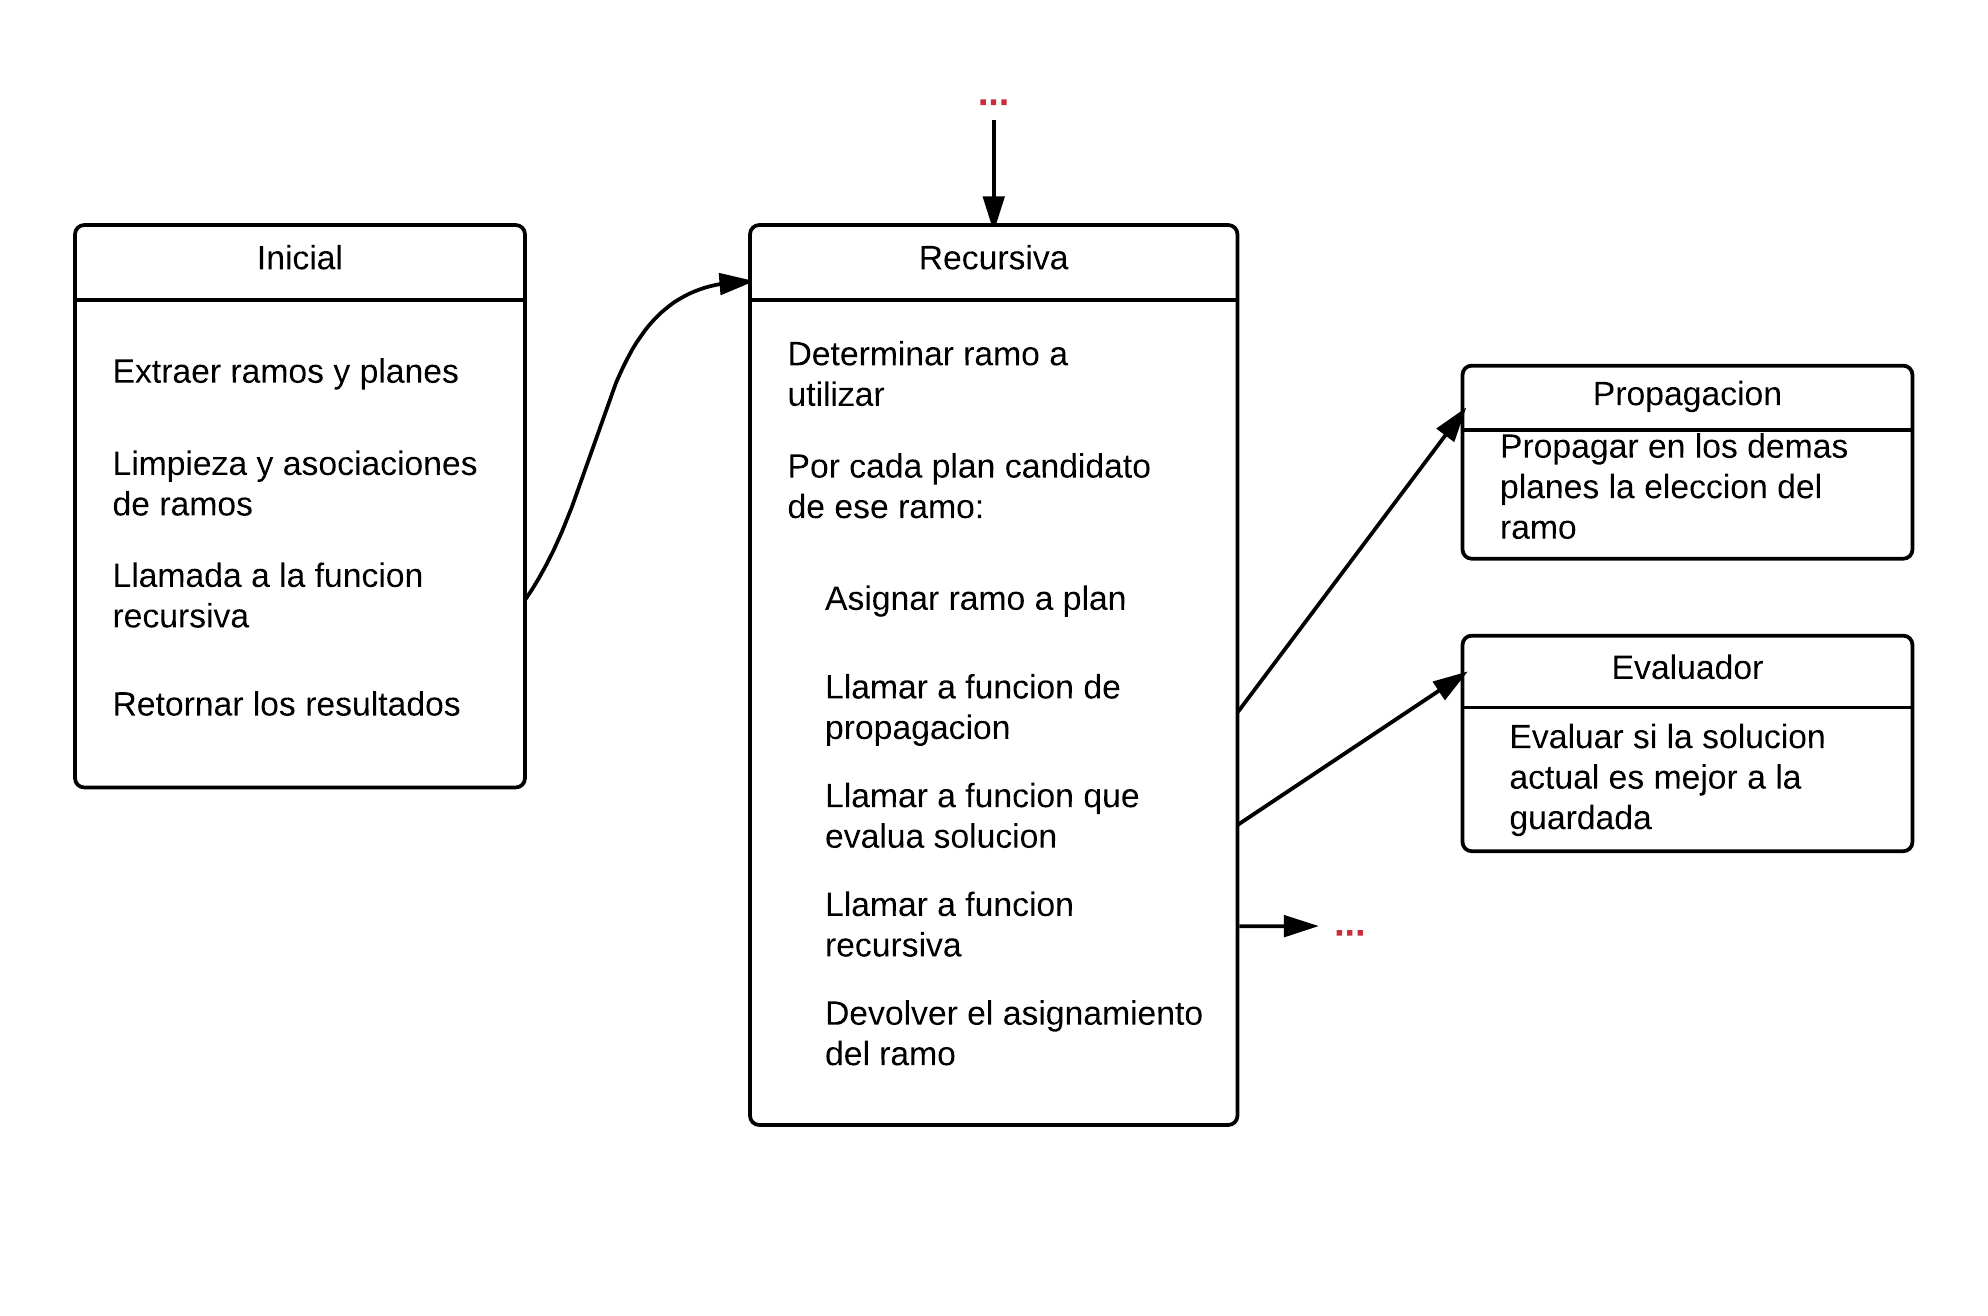
\includegraphics[scale=0.7]{imagenes/15}
	\caption{Funciones de la implementaci�n anterior y sus comportamientos.}
	\label{impl_old}
\end{figure}

En este caso, se utiliz� la misma forma de programaci�n procurando que todas las funciones tuvieran una firma similar entre ellas, respetando que siempre reciban la lista de ramos y planes, y retornen la mejor soluci�n si corresponde. Adem�s, como no estaba dentro del alcance, se reutiliz� la implementaci�n hecha en la funcion inicial de la implementaci�n anterior. Por lo tanto, se poseen seis funciones, donde tres de ellas se corresponden con las explicadas en el p�rrafo anterior exceptuando la recursiva, debido a que se cambi� el comportamiento del algoritmo.

\begin{figure}[!h]
	\centering
	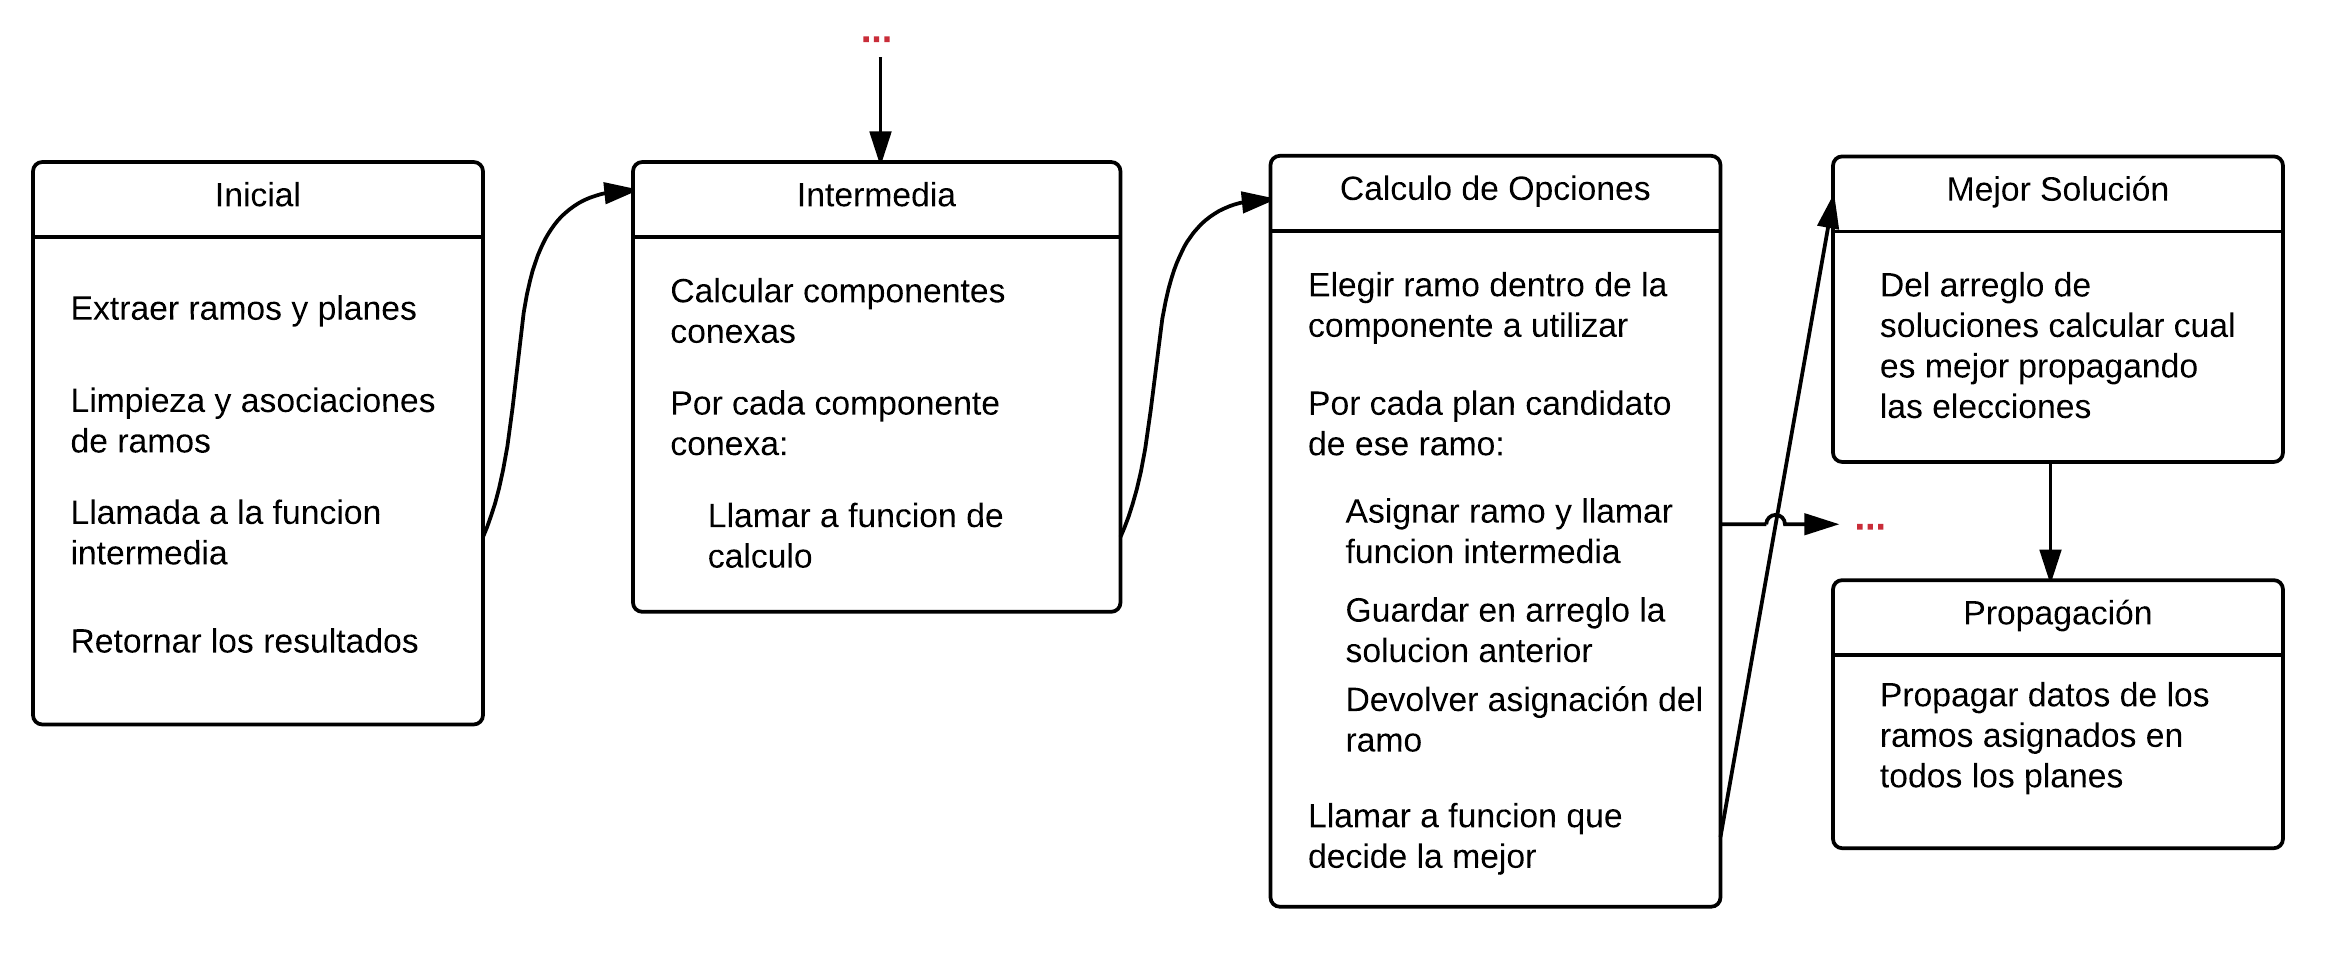
\includegraphics[scale=0.2]{imagenes/16}
	\caption{Funciones de la nueva implementaci�n y sus comportamientos.}
	\label{impl_new}
\end{figure}

Una de las funciones es el c�lculo de las componentes conexas, donde a partir de los ramos se dividen en distintos arreglos debido a los planes que comparten. A esta funci�n siempre se le entrega la lista de todos los ramos y planes, pero puede adicionarse una tercera variable opcional que dice que subconjunto de esas listas deben ser considerados para el c�lculo y cu�les elementos deben quedan fuera.

Otra funci�n es el c�lculo de la mejor soluci�n a partir de un arreglo de soluciones. En ella se recibe un arreglo y en una variable auxiliar se va guardando la mejor mientras se recorre el arreglo. Al t�rmino retorna aquella variable.

La funci�n recursiva de la implementaci�n antigua se cambi� por dos funciones nuevas. La primera es el paso intermedio donde se calculan las componentes conexas y por cada una de ellas se inicia el c�mputo de las distintas opciones de un ramo. La segunda es la que realiza este c�lculo, elige un ramo y eval�a todas sus opciones (llamando a la primera funci�n) generando un arreglo de posibles soluciones el que es pasado al m�todo explicado en el p�rrafo anterior donde se calcula cu�l es mejor.

En la primera funci�n descrita en el p�rrafo anterior es donde debe ir ubicada la implementaci�n del cach�. Alli, se debe encontrar una firma (hash) que diferencie los elementos a guardar en memoria de manera tal de discriminar cu�l componente conexa generada est� repitiendo su c�lculo para ser extraida desde la memoria y no necesitar el llamado a la segunda funci�n.

Finalmente, se posee la funci�n que realiza un recorrido con orden posterior (post order traversal) del �rbol de planes para propagar las elecciones hechas en cada paso del segundo m�todo explicado en el p�rrafo anterior.
 % Implementaci�n
\chapter{Validaci�n}
\lipsum[1-15]
\begin{defn}[ver \cite{KAR00}] Definici�n definitiva $$\frac{d}{dx}\int_a^xf(y)dy=f(x).$$\end{defn}
 % Validaci�n
\begin{conclusion}

A partir de lo ya dicho en la secci�n de ``Validaci�n'', se logr� formular un algoritmo capaz de mejorar la anterior automatizaci�n del recuento de UD's reduciendo considerablemente los tiempos de gran parte de los planes y evidenciar de buena manera el comportamiento que sigue para proximas evaluaciones de los metodos e implementaciones realizadas.

Si bien se encontr� un caso en que el comportamiento no es el �ptimo, se logr� esclarecer las razones constatando c�mo una decisi�n administrativa que afecta la disposici�n de los ramos puede llegar a influir tanto a la descripci�n del avance curricular del alumno como perjudicar el calculo automatizado. 

Como opini�n, se considera que los cambios de la carrera de Ingenier�a Civil Industrial poseen innovaciones en las metodologias o adecuaci�n a las necesidades de los estudiantes, por lo tanto, son medidas atractivas que logran instaurarse dentro del normal desarrollo. Aun as�, debe existir un equilibrio y concenso a nivel de universidad de la instauraci�n de este tipo de medidas en el sentido de que actualmente, como se poseen dominios separados entre departamentos y escuela, se debe velar por el normal funcionamiento local pero a su vez debe existir una cohesi�n para el trabajo en conjunto. Esto incluso implica el asesoramiento que deben tener ciertas implementaciones de normas y reglamentos debido a la falta de visi�n en la posibilidad de implementaci�n que pueden llegar a poseer. Se debe tener cierta certeza de la posibilidad de puesta en marcha antes de firmar un decreto.

Por otra parte, evaluando superficialmente el recuento de UD's en versiones antiguas (por ejemplo en el plan ``Ingenier�a Civil Electricista v2'') se logr� notar ciertos planes que no segu�an un comportamiento logico m�s que el rellenar de alguna manera recuentos que no cumplian todas las reglas (como es el caso de los planes ``Libres''). Esto tambien se debe a que antiguamente el actor principal del proceso tenia la potestad y mayor flexibilidad a la hora de decidir los alumnos con viabilidad de titularse. En cambio, este al ser un sistema automatizado posee mayor rigidez y, si bien en un inicio se poseen planes bien modelados, finalmente se incurre a ``ensuciar'' los planes de estudios a trav�s del tiempo. 

Un ejemplo de esto fue la inclusi�n, hace un tiempo atras, de dos ramos de computaci�n reemplazando el antiguo curso de programaci�n que si bien fue una excelente medida, el modelamiento inicial en el recuento de UD's fue cuestionable y dadas converzaciones termin� ensuciando despreciablemente el plan. Aun as�, recuperando uno de los parrafos mencionados en el ``Marco Te�rico'' acerca de la componente gigante que puede formarse en grafos aleatorios al ir agregando cada vez mas elementos, si bien no es del todo el caso, el ``ensuciar'' de a poco la carrera puede provocar finalmente la generaci�n de una gran componente gigante implicando que parte de las mejoras provocadas en esta memoria debido a la separaci�n de componentes conexas se vea neutralizada.

Por lo anterior, ser�a util la formaci�n de herramientas que permitan guiar y asesorar los lineamientos de los planes de estudios para que si bien permitan innovaciones dentro de �l o la adici�n de elementos creativos, tambien se posea una mirada tecnol�gica con experiencia fundada de la evaluaci�n de dichos planes y vayan analizando a trav�s del tiempo su comportamiento.

\textbf{No se si darle un parrafo a la generalizaci�n que puede darse al recuento en otras facultades como medicina. Generalizar validacion para medi y ver si alcanza el tiempo para agregarlo.}

\end{conclusion}
 % Conclusiones

\bibliographystyle{plain}
\bibliography{bibliografia}

\appendix
\chapter{C�digo de la Implementaci�n}

%Colores PHP
\newcommand{\PHPamountofcolor}{75}
\newcommand{\SourceCodeContext}{5}
\definecolor{PHP_comment_old}{HTML}{CCCCCC}
\colorlet{PHP_comment}{PHP_comment_old!\PHPamountofcolor!black}
\definecolor{PHP_default_old}{HTML}{000000}
\colorlet{PHP_default}{PHP_default_old!\PHPamountofcolor!black}
\definecolor{PHP_keyword_old}{HTML}{6c9c11}
\colorlet{PHP_keyword}{PHP_keyword_old!\PHPamountofcolor!black}
\definecolor{PHP_emph1_old}{HTML}{0F58A2}
\colorlet{PHP_emph1}{PHP_emph1_old!\PHPamountofcolor!black}
\definecolor{PHP_emph2_old}{HTML}{CCAA00}
\colorlet{PHP_emph2}{PHP_emph2_old!\PHPamountofcolor!black}
\definecolor{PHP_emph4_old}{HTML}{C60484}
\colorlet{PHP_emph4}{PHP_emph4_old!\PHPamountofcolor!black}
\definecolor{PHP_string_old}{HTML}{C78F0A}
\colorlet{PHP_string}{PHP_string_old!\PHPamountofcolor!black}
\definecolor{PHP_variable_old}{HTML}{C82210}
\colorlet{PHP_variable}{PHP_variable_old!\PHPamountofcolor!black}
\definecolor{PHP_number_old}{HTML}{BF1CA6}
\colorlet{PHP_number}{PHP_number_old!\PHPamountofcolor!black}
\newtoggle{InString}{}
\togglefalse{InString}
\newcommand*{\ColorIfNotInString}[1]{\iftoggle{InString}{#1}{\color{PHP_number}#1}}
\newcommand{\PHPhighlightvar}[1]{\ifnum\theDollarFlag=1 \color{PHP_variable} \fi#1\setcounter{DollarFlag}{0}}
\newcounter{DollarFlag}

\lstset{
	language				= PHP, 
	breaklines			= true, 
	basicstyle			= \footnotesize, 
	keywordstyle 		= \color{PHP_keyword},
	stringstyle 		= \color{PHP_string!90!black}\toggletrue{InString},
	literate 				= {\$}{{\iftoggle{InString}{\$}{\setcounter{DollarFlag}{1}\color{PHP_variable}\$\color{PHP_default}}}}1
	{0}{{{\ColorIfNotInString{0}}}}1
	{1}{{{\ColorIfNotInString{1}}}}1
	{2}{{{\ColorIfNotInString{2}}}}1
	{3}{{{\ColorIfNotInString{3}}}}1
	{4}{{{\ColorIfNotInString{4}}}}1
	{5}{{{\ColorIfNotInString{5}}}}1
	{6}{{{\ColorIfNotInString{6}}}}1
	{7}{{{\ColorIfNotInString{7}}}}1
	{8}{{{\ColorIfNotInString{8}}}}1
	{9}{{{\ColorIfNotInString{9}}}}1,
	identifierstyle = \color{PHP_default}\PHPhighlightvar,
	commentstyle 		= \color{PHP_comment}\slshape,
	emph 						=[1]{require_once, require, include_once, include, namespace, use, class, function, new},
	emphstyle 			=[1]\color{PHP_emph1},%\bf,
	emph 						=[2]{echo, empty, isset, array, instanceof},
	emphstyle 			=[2]\color{PHP_emph2},%\bf,
	emph 						=[3]{var, const, abstract, protected, private, public, static, final, extends, implements, global, if, else, foreach ,for, endforeach, endif, endfor, elseif, as},
	emphstyle 			=[3]\color{PHP_keyword},%\bf,
	emph 						=[4]{return, throw, exit, __halt_compiler, continue, break},
	emphstyle 			=[4]\color{PHP_emph4},%\bf,
	captionpos 			= b,
	rulecolor 			= \color{black},
	keywords 				= {__halt_compiler, abstract, and, array,as, break, callable, case, catch, class,clone, const, continue, declare, default,die, do, echo, else, elseif, empty, enddeclare, endfor, endforeach, endif, endswitch, endwhile, eval, exit, extends, final, finally, for, foreach, function, global, goto, if, implements, include, include_once, instanceof, insteadof, interface, isset, list, namespace, new, or, print, private, protected, public, require, require_once, return, static, switch, throw, trait, try, unset, use, var, while, xor, yield },
	numbers					= left,
	stepnumber			= 1, 
	numberfirstline	= true,
	numberstyle			= \footnotesize,
	upquote					= true,
	showlines				= true
}

\lstinputlisting[firstline=6,lastline=319]{codigo/api.php}
 % opcionales

\end{document}
